\documentclass[addpoints,12pt]{exam}
%\documentclass[12pt]{article}
\usepackage[letterpaper, margin=0.75in]{geometry}
\usepackage{graphicx}
\usepackage{enumitem}
\usepackage{booktabs}

\begin{document}
\footer{}{Page \thepage\ of \numpages}{}

\begin{flushright}
\makebox[0.5\textwidth]{\large Name:\enspace\hrulefill}
\vspace{0.2in}

\makebox[0.5\textwidth]{\large Date:\enspace\hrulefill}
\end{flushright}

\begin{center}

\includegraphics[width=10cm]{../images/logo.png}
\end{center}

\begin{center}
\noindent{\LARGE Conceptual Physics \\ Reading Quiz 4}
\end{center}

\noindent\begin{large}\textbf{Due Date: March 2 (before class)}\end{large}
\vspace{0.2in}

This reading assignment covers the material that we will discuss and work on next week. Our class activities will \textbf{assume} that you have read the assigned material, therefore it is \textbf{very important} that you do so to get the most out of the class!

Also below is a cartoon picture of the atom, following the atomic model that makes it look like planets:

\noindent \begin{center}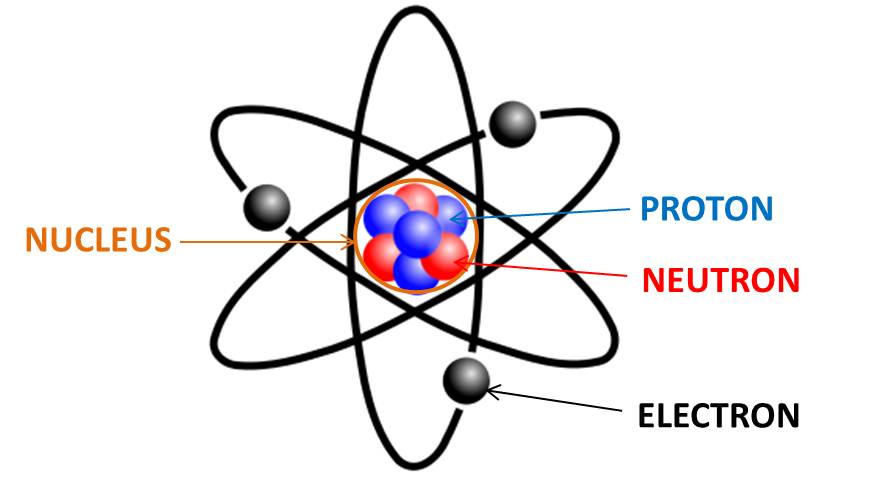
\includegraphics[width=4in]{../images/atom.jpg}\end{center}

Where the \textit{nucleus} is located in the middle of the atom and is orbited by electrons. Protons are \textit{POSIT}ively charged, neutrons carry no charge (\textit{NEUT}ral) and electron are negatively charged (and named for archaic reasons having to due with Greeks and tree resin). Electrons are \textit{fundamental particles} - they cannot (to our knowledge) be further broken down. Protons and neutron, however, are composite particles, meaning that they can be further broken down. \textit{Quarks} come together to form protons and neutrons, and are themselves fundamental particles (discussed in Chapter 0 of \textit{Light and Matter} and chapter 33, section 5 of \textit{College Physics}).

\begin{enumerate}

	\item Handout on \textit{The Fundamental Interactions} in the course reader.
	
	The purpose of this reading is to introduce the (known) fundamental forces of nature. Pay special attention to gravity and the electromagnetic force (in the first 12 pages). It also serves as an introduction to the atom, which will be very handy in part 2 of this course. The section that talks about action at a distance and carrier particles is really cool, but not necessary for next class (we will revisit it again in week 9 when we talk about atomic and particle theory, and again in week 10 when we talk about fields of force, so it's a good introduction but you can skip if you're short on time).
	
	\item \textit{Light and Matter}, Chapter 4 (all Sections)
	
	This chapter introduces forces in the physics technical way. Pay attention to what a force is, and in particular what a force is not (Section 4). It is important to understand what happens when multiple forces act on an object simultaneously.
	
	
\end{enumerate}

As part of the reading, please complete the pre-class quiz \textit{before} coming to class. They will be collected at the very beginning.
 
\clearpage

\begin{flushright}
Score: \hspace{0.2in} / \numpoints ~ points
\end{flushright}

\noindent Questions from handout on 4 Fundamental Interactions (Forces) in course reader

\begin{questions}

\question[1]
What are the four fundamental forces/interactions?
\fillwithlines{0.5in}

\question[1]
The Earth and an apple each exert a gravitational force on each other that pulls them together. If the mass of the apple doubled, how would this force change (increase, decrease, or stay the same)?
\fillwithlines{0.5in}

\question[1]
Do like charges attract or repel each other? What about opposite charges?
\fillwithlines{0.75in}

\question[1]
What force binds the nuclei of atoms together? \fillwithlines{0.5in}

\question[1]
In our everyday life, we encounter \textit{contact} forces that, for example, allow us to push down on a table with our hand without it passing through the table. What is responsible for these contact forces?
\fillwithlines{0.5in}

\end{questions}

\noindent Questions from \textit{Light and Matter} Chapter 4

\begin{questions}
\question[1]
Do forces cause motion, or cause changes in motion?
\fillwithlines{0.5in}

\question[1]
What is Newton's First law?
\fillwithlines{0.5in}

\question[1]
What happens to an object if the total forces acting on it are not zero? (hint: see section 4, Newton's second law)
\fillwithlines{0.5in}

\question[1]
What is an \textit{inertial frame of reference}?
\fillwithlines{0.5in}

\question[1]
What principle is violated in non-inertial frames of reference?
\fillwithlines{0.5in}

\end{questions}


\end{document}